\documentclass[10pt]{article}
\usepackage[utf8]{inputenc}
%\usepackage[T1]{fontenc}
\usepackage{tgbonum}
\usepackage[english]{babel}
\usepackage{graphicx}
\usepackage{amsmath}
\usepackage{amssymb}
\usepackage{hyperref}
\usepackage{epsf}
\usepackage{float}
\usepackage{mathpazo}
\usepackage
[
a4paper,% other options: a3paper, a5paper, etc
left=2.2cm,
right=2.2cm,
top=3cm,
bottom=3cm,
]{geometry}
%\geometry{hmargin=3.5cm, vmargin=2.5cm}
\usepackage{fancyhdr}
\pagestyle{fancy}
\fancyhf{}
\rfoot{\thepage}
\renewcommand{\headrulewidth}{0pt}
\usepackage{color}
\graphicspath{{DWGs/}}
\usepackage{graphicx}
\usepackage{wrapfig}
\usepackage{graphicx}
\usepackage{multicol}
\usepackage{enumitem}
\usepackage{xcolor}
\usepackage{framed}
\definecolor{shadecolor}{RGB}{139, 231, 3}
\usepackage{epigraph}

\usepackage{tcolorbox}
\definecolor{mycolor}{rgb}{0.122, 0.435, 0.698}

\usepackage{anyfontsize}
\usepackage{t1enc}

\begin{document}


\setlength{\parskip}{0.6em}
\setlength{\parindent}{0cm}

This document was prepared as part of the course \textit{The Basics of Transport Phenomena} from Delft University of Technology, available on edX.org as DelftX: TP101x.

\section*{Conduction in a rod with internal heat production}

This is a derivation of the temperature distribution function $T(x)$ for a steady-state heat conduction in a straight rod of length $L$. We assume that the internal heat production $Q_p$ is present in every point inside the rod volume (which may simulate heating of an electrical wire). The rod is perfectly insulated along its length and it loses heat only through its endpoints which in a steady-state case are kept at a fixed temperature $T_0$.

We will take for the control volume a slice $dx$ from the rod. 

The energy balance for the rod element:

\begin{equation}
\frac{dE}{dt} = E_{in} - E_{out} + E_{production}
\end{equation}

(note here that $E_{in}$, $E_{out}$ and $E_{production}$ are energies per unit time and so have the units of $\frac{J}{s}$)

The heat flow is described by the Fourier's law:

\begin{equation}
\phi = \lambda A \Big(- \frac{dT}{dx} \Big)
\label{eq:fourier}
\end{equation}

Hence:

\begin{equation}
E_{in} = \lambda A \Big(- \frac{dT}{dx} \Big)_x
\end{equation}

\begin{equation}
E_{out} = \lambda A \Big(- \frac{dT}{dx} \Big)_{x + dx}
\end{equation}


The energy per unit time coming from the production can be written as $Q_p$ (which is in the units of $\frac{W}{m^3}$) multiplied by the volume of the slice $dx$:

\begin{equation}
E_{production} = Q_p A dx
\end{equation}

In the steady-state $\frac{dE}{dt} = 0$ and the energy balance becomes:


\begin{equation}
\lambda A \Big(- \frac{dT}{dx} \Big)_x - \lambda A \Big(- \frac{dT}{dx} \Big)_{x + dx} + Q_p A dx = 0
\end{equation}

Simplifying the above energy balance we get:

\begin{equation*}
\frac{\Big(\frac{dT}{dx} \Big)_{x + dx} - \Big(\frac{dT}{dx} \Big)_x  }{dx} = - \frac{Q_p}{\lambda}
\end{equation*}

If we now substitute some function $f(x) = \frac{dT}{dx}$ we notice that we have:

\begin{equation*}
\frac{f(x + dx) - f(x)}{dx} = - \frac{Q_p}{\lambda}
\end{equation*}

\newpage

in other words:

\begin{equation}
\frac{df(x)}{dx} = - \frac{Q_p}{\lambda}
\end{equation}

With the above substitution, the differential equation that we are about to solve becomes:

\begin{equation}
\frac{d^2T}{dx^2} = - \frac{Q_p}{\lambda}
\end{equation}

The solution to the above differential equation is:

\begin{equation}
T(x) = - \frac{Q}{2 \lambda} (x^2 - Lx) + T_0
\label{eq:solution}
\end{equation}

It is interesting to note here that the solution does not depend on the cross-sectional surface area of the rod.




\subsection*{Computational example}

As a computational example we will draw the graph of the temperature distribution in a copper rod $200 m$ long. We take that the thermal conductivity for this rod is $400 \frac{W}{m \cdot ^o C}$. The internal heat production is $20 W$.

\begin{figure}[H]
\centering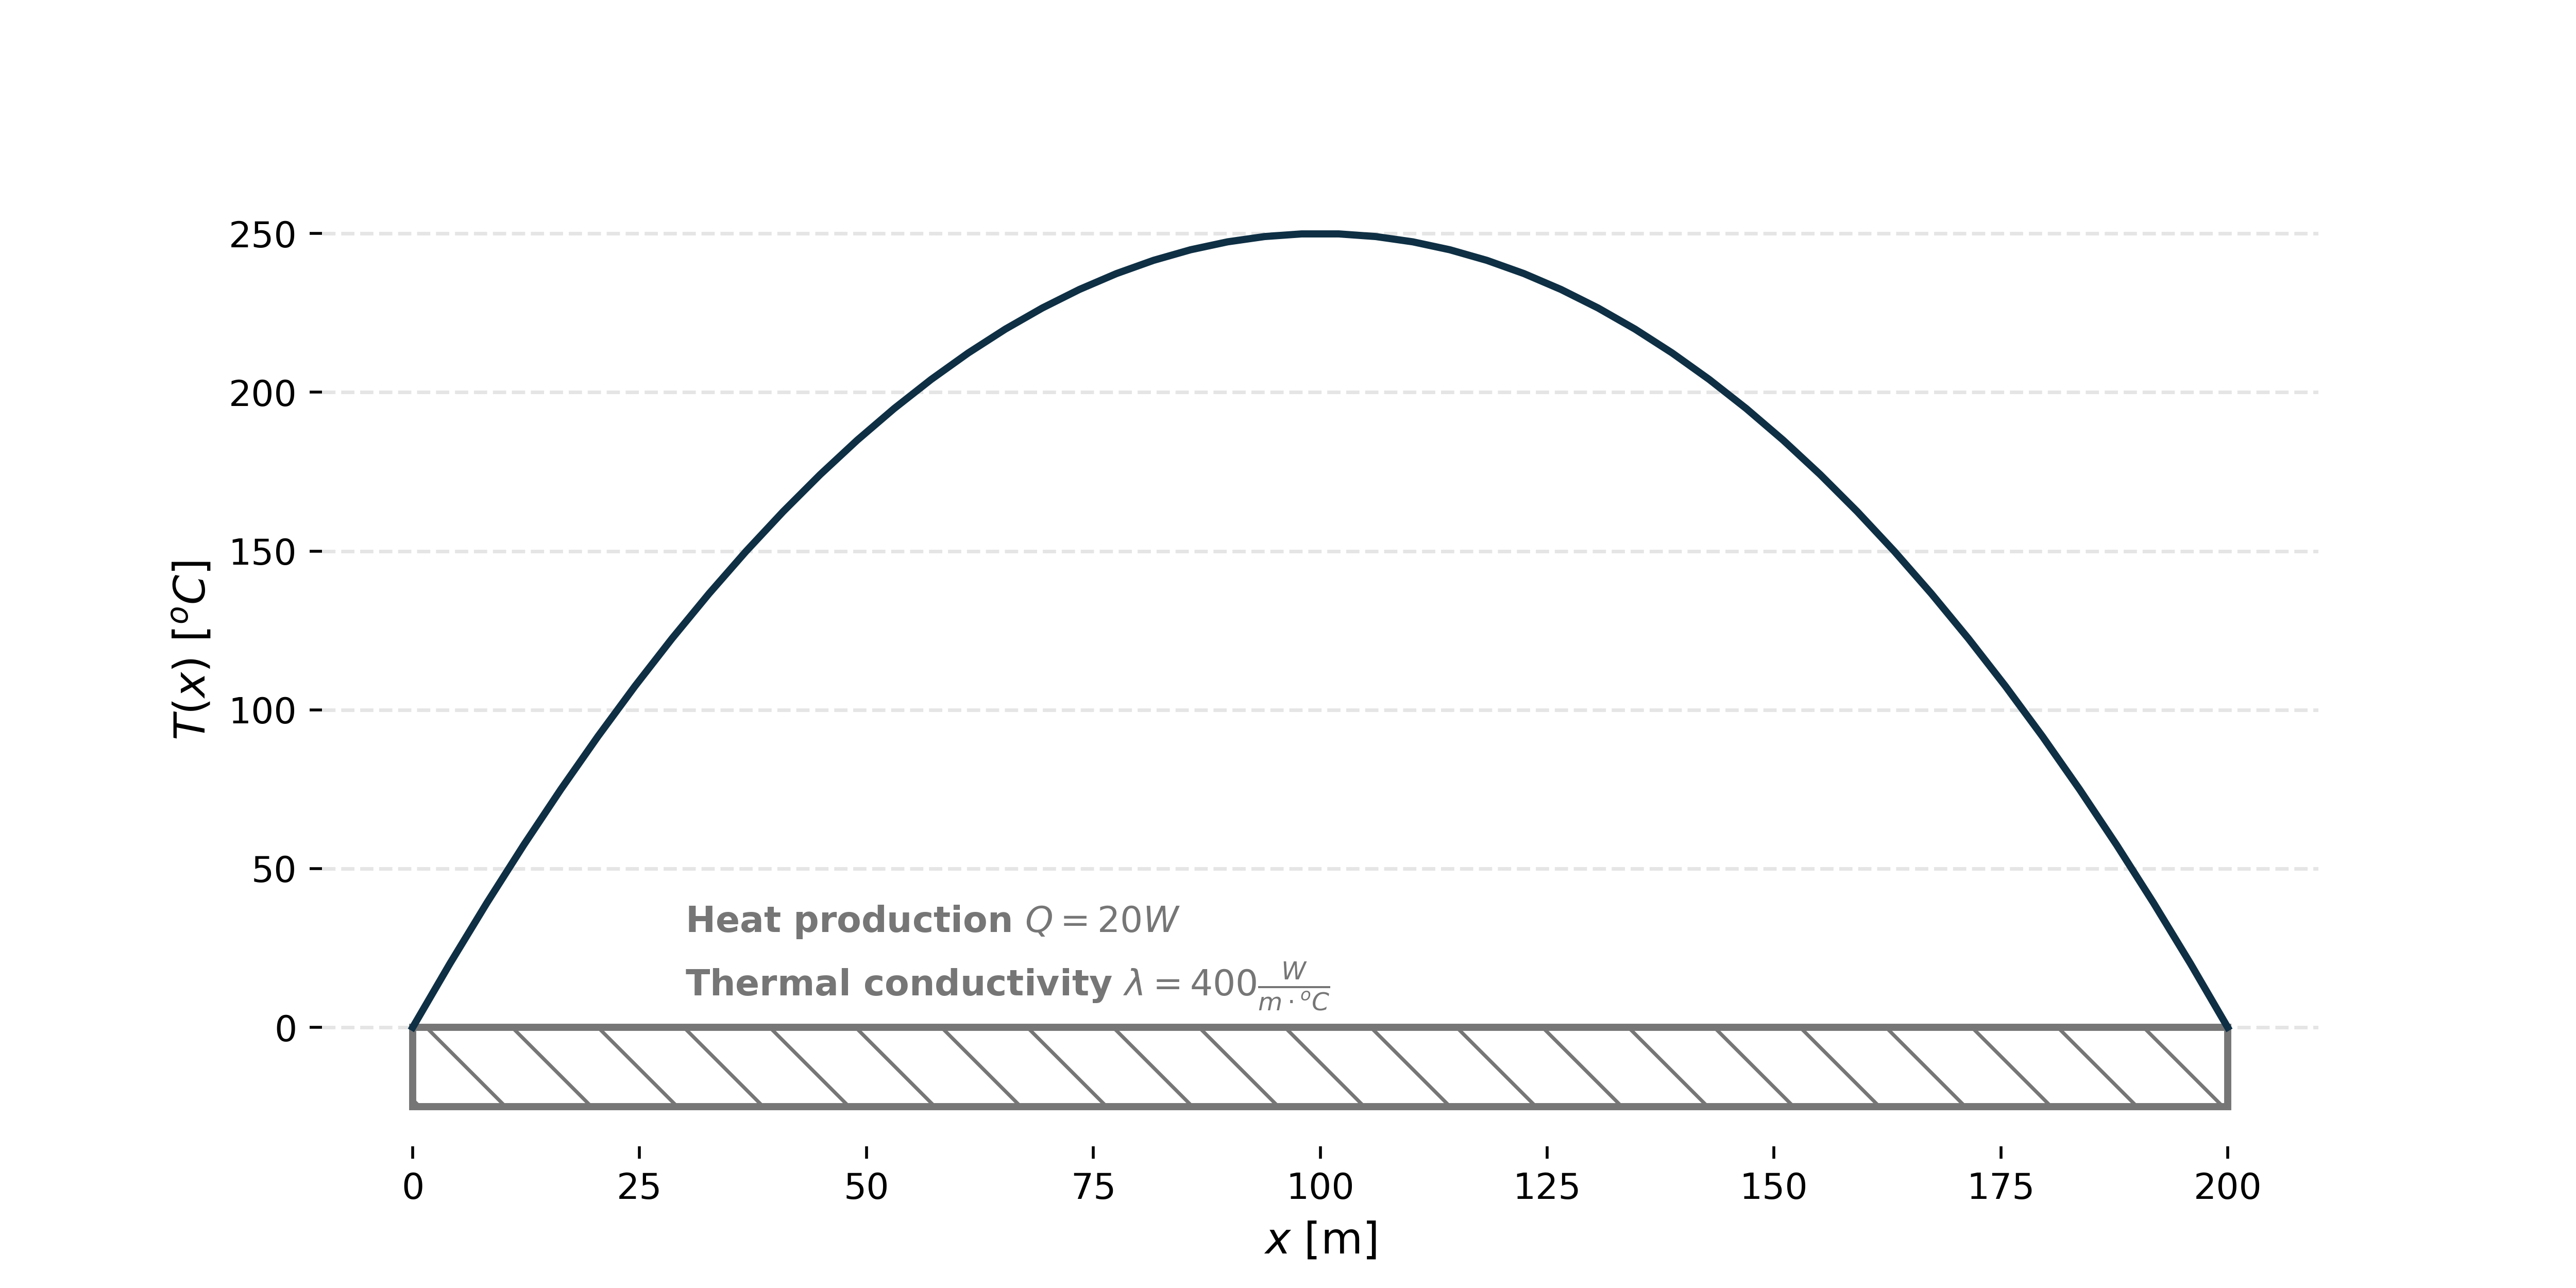
\includegraphics[width=18cm]{temperature_distribution.png}
\caption{Temperature distribution in a rod with internal heat production of $20 W$}
\label{fig:learning_curve}
\end{figure}



\newpage

\thispagestyle{empty}


This material was created by or adapted from material posted on the DelftX website, delftx.tudelft.nl, and created by TU Delft faculty members Robert Mudde, Professor of Multiphase Flow at the Dept. of Chemical Engineering and Peter Hamersma, Associate professor at the Dept. of Chemical Engineering, 2015. DelftX is not responsible for any changes made to the original materials posted on its website and any such changes are the sole responsibility of Kamila Zdybał.

The course materials by Delft University of Technology are subjected to copyright and are licensed under a Creative Commons Attribution-NonCommercial-ShareAlike 4.0 International License.

https://creativecommons.org/licenses/by-nc-sa/4.0/

\begin{center}
\vspace*{7cm}

\setlength{\parskip}{0.0em}
\setlength{\parindent}{0cm}

Copyright \textcopyright \, K. Zdybał, 2018

For more projects similar to this one

visit me on GitHub: \verb|@camillejr|

\verb|camillejr.github.io/science-docs/|

To contact me personally drop me a line at:

\verb|kamilazdybal@gmail.com|

\vspace*{2cm}

\verb|Conduction in a rod with internal heat production|

Typeset with \LaTeX

\vspace*{1.8cm}

\noindent This work is licensed under the Creative Commons

Attribution-NonCommercial-ShareAlike 4.0 International 

(CC BY-NC-SA
4.0) license.
\end{center}

\end{document}